\begin{frame}{The Variational Approximation}

Let $\theta$ be unknown parameters and $y$ the data.

We posit a class of mean-field distributions parameterized by a real vector $\eta$.

We solve
\begin{align*}
  \eta^* = \argmin_{\eta} KL\left(
      q(\theta \vert \eta )\big\| p(\theta | y)
      \right)
\end{align*}

\only<1>{
\begin{figure}[!h]
\centering
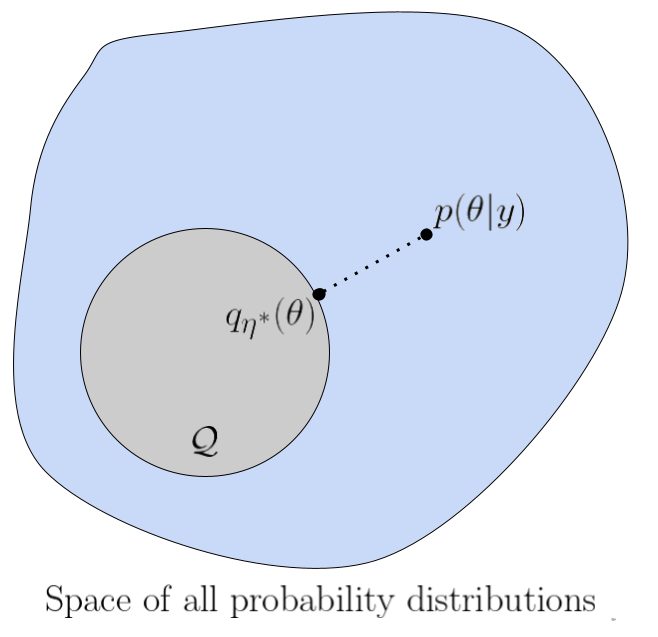
\includegraphics[width = 0.4\textwidth]{./figures/vi_schematic2.png}
\end{figure}
}

\only<2->{
Note that

\begin{itemize}
\item The optimal variational parameters $\eta^*$ depend on the prior through optimizing the KL objective.

\pause

\item The approximate posterior quantities are then functions of $\eta^*$, e.g.\
\begin{align*}
\eta^* \mapsto
\Expect_{q_{\eta^*}} \left[ \#\text{clusters} \right]
\quad \text{ or } \quad
\eta^* \mapsto
\Expect_{q_{\eta^*}}
\left[\#\{\substack{\text{clusters in}\\\text{new dataset}}\} \right].
\end{align*}

\end{itemize}
}

\only<3>{
\begin{mdframed}[style=MyFrame]
\begin{center}
{\bf How do these approximate posterior quantities depend on the DP prior?}
\end{center}
\end{mdframed}
}
\end{frame}
